


\section{Nichtlineare Optimierung}

\textbf{Satz von Schwarz:\skript{2}} $\frac{\partial^2 f(x_1, x_2)}{\partial x_1 \partial x_2} = \frac{\partial^2 f(x_1, x_2)}{\partial x_2 \partial x_1}$\\
Bei partiellen Ableitungen spielt die Reihenfolge keine Rolle. (Bedingung: Alle partiellen Ableitungen stetig.)

\begin{minipage}[t]{0.4\linewidth}
\subsection{Gradient\skript{3}}
Der Gradient zeigt immer in Richtung des steilsten Anstiegs der Funktion $f$ und steht senkrecht auf den Höhenlinien.\\


$\nabla f =\begin{bmatrix}
f_{x_1}\\
f_{x_2}\\
\vdots\\
f_{x_n}
\end{bmatrix}=\begin{bmatrix}
\partFrac{f}{x_1}\\[0.1cm]
\partFrac{f}{x_2}\\[0.1cm]
\vdots\\[0.1cm]
\partFrac{f}{x_n}
\end{bmatrix}$
\end{minipage}
\hfill
\begin{minipage}[t]{0.58\linewidth}
	\subsection{Algebraisch Extrema bestimmen}
	\textbf{Alle Ränder müssen seperat ansgeschaut werden!!!}\\
	(Randwerte einsetzen, dann in verbliebene Richtungen ableiten)\\
	
	\boxed{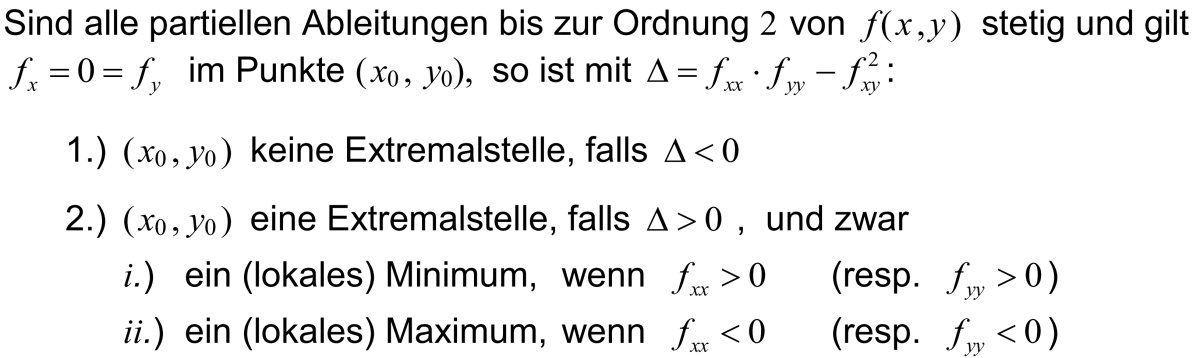
\includegraphics[width=0.9\linewidth]{./Content/NonLinearOptimization/maxMin}}\\
\end{minipage}



  \begin{minipage}[t]{8.5cm}
 \subsection{Gradientenverfahren\skript{4}}
    Von der Stelle $\vec{x}^{(i)}$ wird in Richtung des Antigradienten geschritten. 
    $$\vec{x}^{(i+1)} = \vec{x}^{(i)} - \alpha_i \nabla f(\vec{x}^{(i)})$$
\subsubsection{Eigenschaften}    
    Vorteile:
    \begin{liste}
      \item Einfach zu implementieren
      \item Findet optimale Lösung
      \item Keine gute Startnäherung nötig
    \end{liste}
    
    Nachteile:
    \begin{liste}
      \item Konvergiert langsam
      \item In der Nähe der optimalen Lösung Zick-Zack-Kurs
    \end{liste}
    
    \subsubsection{Algorithmus (zur Minimierung)}
  \end{minipage}
  \hfill
  \begin{minipage}[t]{10cm}
  	  \subsection{Differential-Rechnung}
  	  $f'(x_0)=\lim\limits_{\Delta x\rightarrow 0}
  	  \frac{f(x_0+\Delta)x-f(x_0)}{\Delta x}$\\
  	  	\begin{tabular}{llll}
  	  		Kettenregel:	& $\Bigl(f\big(g(x)\big)\Bigr)'$ &$=$ & $g'(x)\cdot f'\big(g(x)\big)$\\[0.1cm]
  	  		%oder $\frac{d f(g(x))}{dx} = f'(g(x)) \cdot g'(x)$\\[0.1cm] 
  	  		Produktregel:	& $\Bigl(f(x)\cdot g(x)\Bigr)'$ &$=$ & $f'(x)\cdot g(x) + f(x)\cdot g'(x)$\\[0.1cm]
  	  		Quotientenregel:& $\left(\frac{f(x)}{g(x)}\right)'$ &$=$ & $\frac{f'(x)g(x)-f(x)g'(x)}{g^2(x)}$\\
  	  	\end{tabular}
	  \begin{minipage}{4.5cm}
	    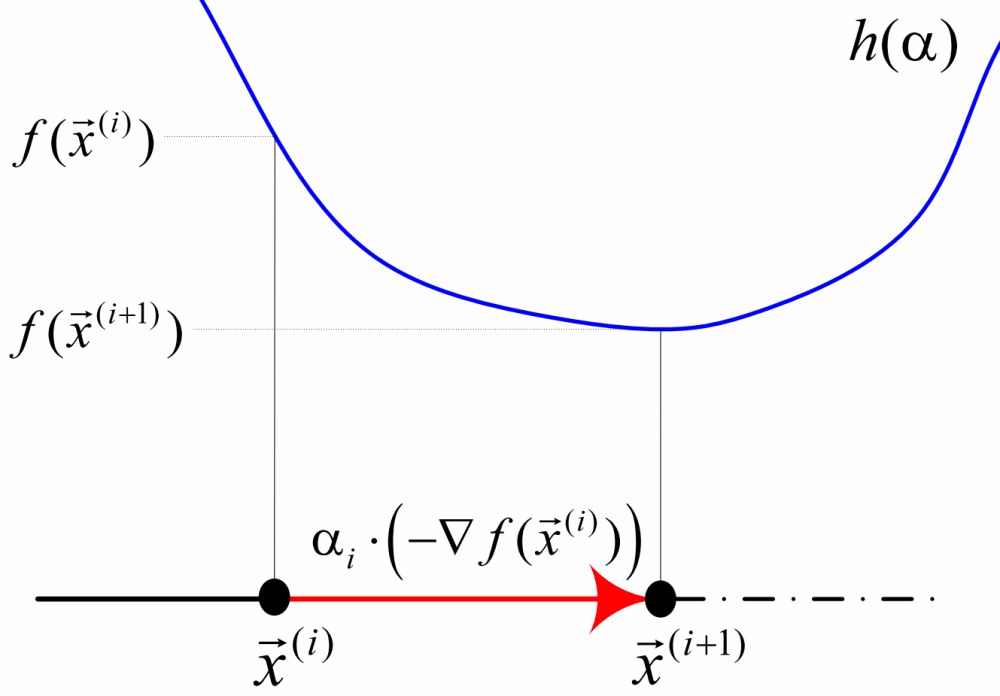
\includegraphics[width=4.5cm]{./Content/NonLinearOptimization/Gradient1D.png}
	  \end{minipage}
	  \hfill
	  \begin{minipage}{4.5cm}
	  	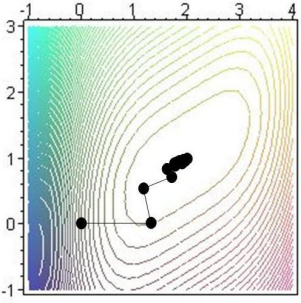
\includegraphics[width=4.5cm]{./Content/NonLinearOptimization/gradient-descent}
	  \end{minipage}
 \end{minipage}
 
 
 
 \begin{enumerate}
	\item $\beta_1=0$\quad$\beta_3=1$\qquad$h(\beta_i)=f\Bigl(\vec{x}^{(i)} - \beta_i \nabla f(\vec{x}^{(i)})\Bigr)$
	\item $while\Bigl(h(\beta_3)\geq h(\beta_1)\Bigl)\Bigl\{\beta_3=\frac{\beta_3}{2}\Bigr\}$
	\item Parabel konstruieren: $P(\beta)=A\beta^2+B\beta+C$\quad mit \quad $\beta_1=0$,\quad $\beta_2=\beta_3/2$\\
		$\begin{bmatrix}
		\beta_1^2 & \beta_1 & 1\\
		\beta_2^2 & \beta_2 & 1\\
		\beta_3^2 & \beta_3 & 1
		\end{bmatrix}\cdot\begin{bmatrix}A\\B\\C\end{bmatrix}=\begin{bmatrix}h(\beta_1)\\ h(\beta_2)\\ h(\beta_3)\\\end{bmatrix}\quad\Rightarrow\quad\begin{bmatrix}
		0 & 0 & 1\\
		\beta_3^2/4 & \beta_3/2 & 1\\
		\beta_3^2 & \beta_3 & 1
		\end{bmatrix}\cdot\begin{bmatrix}A\\B\\C\end{bmatrix}=\begin{bmatrix}h(0)\\ h(\beta_3/2)\\ h(\beta_3)\end{bmatrix}\quad\Rightarrow\quad
		\begin{bmatrix}A\\B\\C\end{bmatrix}=\begin{bmatrix}
		\frac{2h(\beta_1)-4h(\beta_2)+2h(\beta_3)}{\beta_3^2}\\[0.2cm]
		\frac{-3h(\beta_1)+4h(\beta_2)-h(\beta_3)}{\beta_3}\\[0.1cm]
		h(\beta_1)\end{bmatrix}$
  	\item $if\Bigl( (h(\beta_3) = P(\beta_3))\leq-B/2A\Bigr)\Big\{\hat{a}=\beta_3\Big\}$\\
  	$else\Big\{\hat{a}=-B/2A\Big\}$
  	\item $\vec{x}^{(i+1)} = \vec{x}^{(i)} - \hat{a}\nabla f(\vec{x}^{(i)})\quad\Rightarrow\quad $Punkt $ 1.$
  	
  	
 \end{enumerate}
 
 \subsubsection{Matlab-Implementation (nur ein Loop)}
  \begin{MatlabCode}
    % Find betas
    beta1 = 0;
    beta3 = 2; % will be divided by 2 in the loop -> start value = 1
    h_beta1 = subs(f, x, p);
    h_beta3 = 2*h_beta1; % must be higher than h_beta1 (initial)
    while h_beta1 <= h_beta3;
        beta3 = beta3 / 2;
        h_beta3 = subs(f, x, p - beta3 * gradf_numeric);
    end;
    beta2 = beta3/2;
    h_beta2 = subs(f, x, p - beta2 * gradf_numeric);

    % Parabola
    C = h_beta1;
    A = (h_beta3-2.0*h_beta2+C)/(2*beta2*beta2);
    B = (h_beta2-C)/beta2 - beta2*A;
 
    % Candidates for a
    a1 = -B / (2*A);
    a2 = beta3;
    
    % Select a
    if subs(f, x, p - beta3*gradf_numeric) <= h_beta3 
        a = a1;
    else
        a = a2;
    end
    
    
    % Calculate next step
    p = p - a * gradf_numeric;
  \end{MatlabCode}
  
\subsection{Newton-Verfahren\skript{7}}

  \begin{minipage}{13cm}
  	\textbf{Tangentengleichung:}\\
  	$t(x^{(i+1)})=f(x^{(i)})+f'(x^{(i+1)})\cdot(x^{(i)})=0\quad\Rightarrow\quad x^{(i+1)}=x^{(i)}-\frac{f(x^{(i)})}{f'(x^{(i)})}$\\
  	
  	\textbf{Bestimmung der Ableitung (numerisch):}\\
  	$f'(x^{(i)})\approx\frac{f(x^{(i)}+h)-f(x^{(i)})}{h}\qquad$ für $h<<1$\\
  	
    Anstelle des Gradienten wird eine Tangente an den Arbeitspunkt gelegt.
    $$\vec{x}^{(i+1)} = \vec{x}^{(i)} - \left(\bm H(\vec{x}^{(i)})\right)^{-1} \nabla f(\vec{x}^{(i)})$$
    mit der Hesse-Matrix
    $$\bm{H}(\vec{x})=
    \left(\frac{\partial^2f}{\partial x_i\partial x_j}(x)\right)_{i,j=1,\dots, n}=
    \begin{pmatrix}
    \frac{\partial^2 f}{\partial x_1\partial x_1}(x)&\frac{\partial^2 f}{\partial x_1\partial x_2}(x)&\cdots&\frac{\partial^2  f}{\partial x_1\partial x_n}(x)\\[0.5em]
    \frac{\partial^2 f}{\partial x_2\partial x_1}(x)&\frac{\partial^2 f}{\partial x_2\partial x_2}(x)&\cdots&\frac{\partial^2  f}{\partial x_2\partial x_n}(x)\\
    \vdots&\vdots&\ddots&\vdots\\
    \frac{\partial^2 f}{\partial x_n\partial x_1}(x)&\frac{\partial^2 f}{\partial x_n\partial x_2}(x)&\cdots&\frac{\partial^2  f}{\partial x_n\partial x_n}(x)
    \end{pmatrix}$$
    (4 Funktionsaufrufe für Diagonalelemente, sonst 3 Funktionsaufrufe)\\
    
    Vorteile:
    \begin{liste}
      \item Gutes Konvergenzverhalten
    \end{liste}
    
    Nachteile:
    \begin{liste}
      \item Hesse-Matrix benötigt zweite Ableitung (numerisch aufwendig)
      \item Inversion der Matrix skaliert schlecht ($O(n^3)$)
    \end{liste}
  \end{minipage}
  \begin{minipage}{6cm}
  	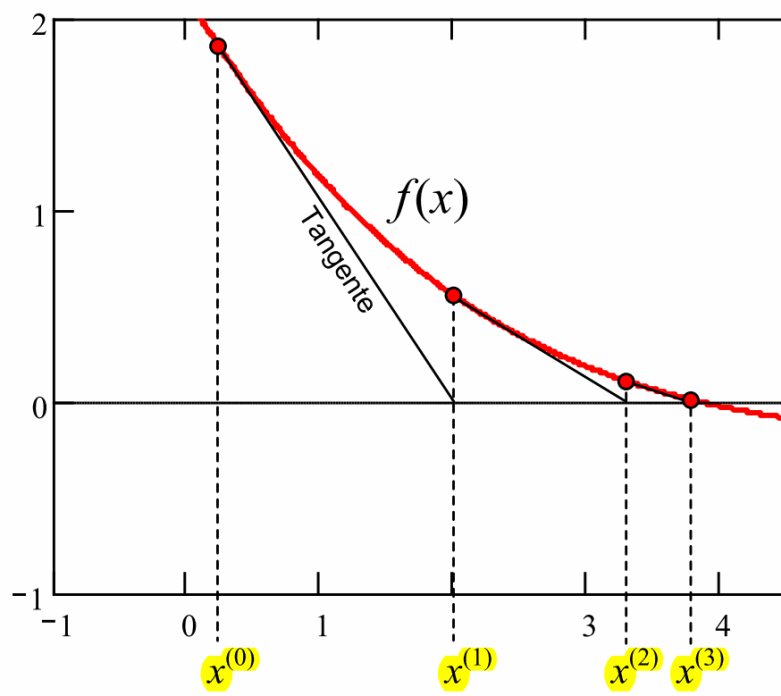
\includegraphics[width=6cm]{./Content/NonLinearOptimization/Newton1D.png}
    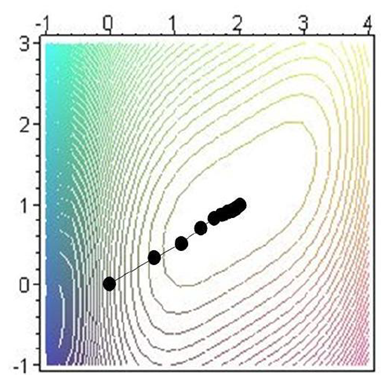
\includegraphics[width=6cm]{./Content/NonLinearOptimization/newton.png}
  \end{minipage}
  
  
\subsection{Quasi-Newton-Verfahren\skript{11}}
  \begin{minipage}{13cm}
  \textbf{Idee:} Die Ableitung des Newton-Verfahren wird durch die Sekantensteigung ersetzt.\\
  
  $F'(x^{(i+1)})\approx\frac{F'(x^{(i+1)})-F'(x^{(i)})}{x^{(i+1)}-x^{(i)}}$\\
  
 \begin{enumerate}
 \item \textbf{Ein Schritt Newton-Verfahren:}
	 \begin{enumerate}
	 \item[(a)] Hesse-Matrix bestimmen: $\mathbf{H}(\vec{x}^{(0)})$\\
	 Gradient bestimmen: $\nabla f(\vec{x}^{(0)})$
	 \item[(b)] $\mathbf{A}_{0}^{-1}=\bigl(\mathbf{H}(\vec{x}^{(0)})\bigr)^{-1}$
	 \item[(c)] $\vec{x}^{(1)}=\vec{x}^{(0)}-\mathbf{A}_{0}^{-1}\cdot\nabla f(\vec{x}^{(0)})$\\
	 \end{enumerate}
 \item $\vec{y}_i=\nabla f(\vec{x}^{(i)})-\nabla f(\vec{x}^{(i-1)})\qquad \vec{s}_i=\vec{x}^{(i)}-\vec{x}^{(i-1)} \qquad i\geq 1$
 \item $\mathbf{A}_{i}^{-1}=\mathbf{A}_{i-1}^{-1}-\displaystyle\frac{\bigl(\mathbf{A}_{i-1}^{-1}\cdot \vec{y}_i-\vec{s}_i\bigr)\vec{s}_i\,^T\cdot \mathbf{A}_{i-1}^{-1}}{\vec{s}_i\,^T\cdot \mathbf{A}_{i-1}^{-1}\cdot\vec{y}_i}\qquad i\geq 1$\\
 \item $\vec{x}^{(i+1)}=\vec{x}^{(i)}-\mathbf{A}_{i}^{-1}\cdot\nabla f(\vec{x}^{(i)})$\qquad zu Punkt 4.
 \end{enumerate}
 
\end{minipage}
\begin{minipage}{6cm}
   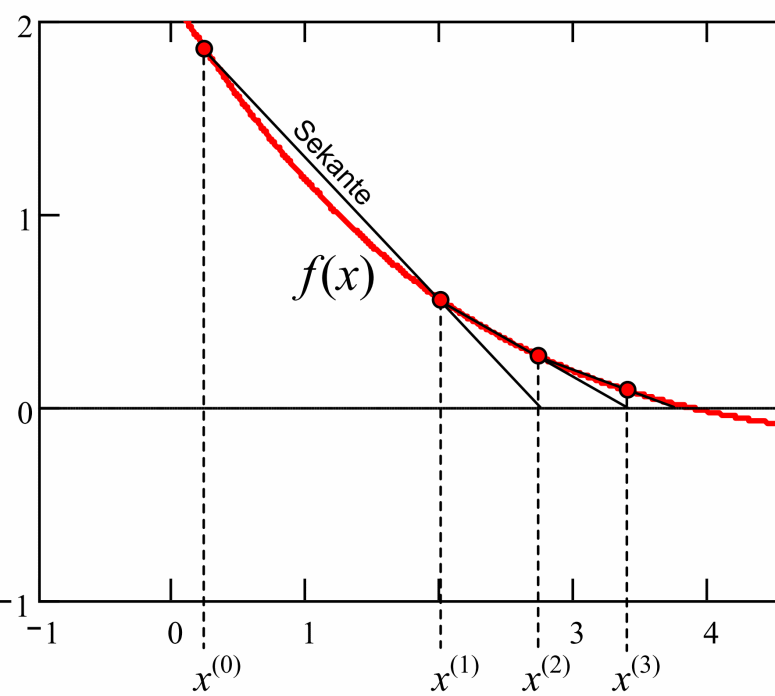
\includegraphics[width=6cm]{./Content/NonLinearOptimization/QuasiNewton1D.png}
   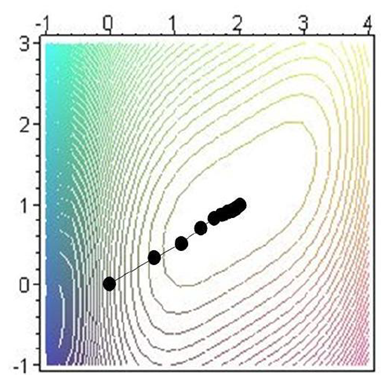
\includegraphics[width=6cm]{./Content/NonLinearOptimization/newton.png}
\end{minipage}


  Um die Berechnung der Ableitungen zu umgehen, werden diese durch finite Differenzen approximiert. 
  $$\frac{\partial^2 f}{\partial x_i^2} = \frac{1}{\epsilon^2} 
  \left( f(x_1, x_2, \ldots, x_i+\epsilon, \ldots, x_n) - 2 f(x_1, x_2, \ldots, x_i, \ldots, x_n) + f(x_1, x_2, \ldots, x_i-\epsilon, \ldots, x_n) \right)$$
  $$\frac{\partial^2 f}{\partial x_i \partial x_j} = \frac{1}{4 \epsilon^2} \begin{pmatrix}
    f(x_1, x_2, \ldots, x_i+\epsilon, \ldots, x_k+\epsilon, \ldots, x_n) - f(x_1, x_2, \ldots, x_i-\epsilon, \ldots, x_k+\epsilon, \ldots, x_n)\\
    -f(x_1, x_2, \ldots, x_i+\epsilon, , \ldots x_k-\epsilon, \ldots, x_n) + f(x_1, x_2, \ldots, x_i-\epsilon, \ldots, x_k-\epsilon, \ldots, x_n)
  \end{pmatrix}$$
 
 \subsection{Konvergenzbeschleunigung\skript{17}}
 \textbf{Idee:} Mit der sogenannten Aitken'sche   $\nabla^2$–Methode wird aus der Folge $\{x_i\}$ die die schneller konvergierende Folge $\{\hat{x}_i\}$ berechnet.\\
 
 Aitken $\nabla^2$-Methode:\quad $\boxed{\hat{x}=x_i-\frac{(x_{i+1}-x_i)^2}{x_{i+2}-2x_{i+1}+x_{i}}}$\qquad $i\geq 0$ \qquad (Formel dimensionsweise anwenden, für $x_1$, $x_2$, $\ldots$)
 
 
 

  
